
\section{Libraries and executables}
\label{sec:libraries}

\subsection{Libraries}

The libraries of this project are currently broken down by task into the following modules:

\begin{enumerate}
     \item Utilities - Commonly used utilities (e.g. date handling, profile timers, etc.)
     \item Math - Math routines: linear algebra, minimizers, interface to optional 3rd-party math libraries (FFTW,GSL).
     \item Message - Controls the topic and verbosity level of application messages/logs to user.
     \item Containers - In-memory data containers of visibility and meta-data and native format I/O.
     \item MK4Interface - Allows for import/export to legacy MK4-types for testing and backwards compatibility.
     \item Operators - Base classes for data manipulation, and generic operations (array reduction, summation, transposition, FFT, etc.).
     \item VLBI - VLBI task-specific data operators (e.g. band-pass correction, per-channel phase offsets, etc.)
     \item Bindings - Python interface to C++ data containers and operators. Allows for python script configuration of data 
     operators at initialization, and user-defined direct access/manipulation of the data.
    \item  Legacy c-libraries (made available for re-use and backwards compatibility and to provide the legacy fourfit application)
    \begin{enumerate}
        \item mk4util - utility library for MK4 data types
        \item dfio - I/O for MK4 data types
        \item afio - I/O library for alist manipulation
        \item ffcontrol - parse old-style fourfit control files 
        \item ffcore - core parameter structures
        \item ffio - output for fringe file data
        \item ffmath - trivial math routines used by fourfit
        \item ffplot - fringe-plot generation library 
        \item ffsearch - core fringe-search algorithm library (grid-search)
    \end{enumerate}
\end{enumerate}

An additional set of plugin libraries will be enabled if the appropriate dependencies are present at compile time, as follows:

 \begin{enumerate}
    \item DIFXInterface - depends on difxio and converts the correlator data into the native data container format.
    \item HDF5 I/O - Converts the native data objects to/from an archival HDF5 file.
    \item Plotting - Utilities to generate plots for data exploration (e.g. fringe-plots). This will be implemented in python.
    \item SIMD extensions (OpenCL) - Parallel implementation of some set of the data operators.
 \end{enumerate}


\begin{figure}[h!]
\begin{center}
  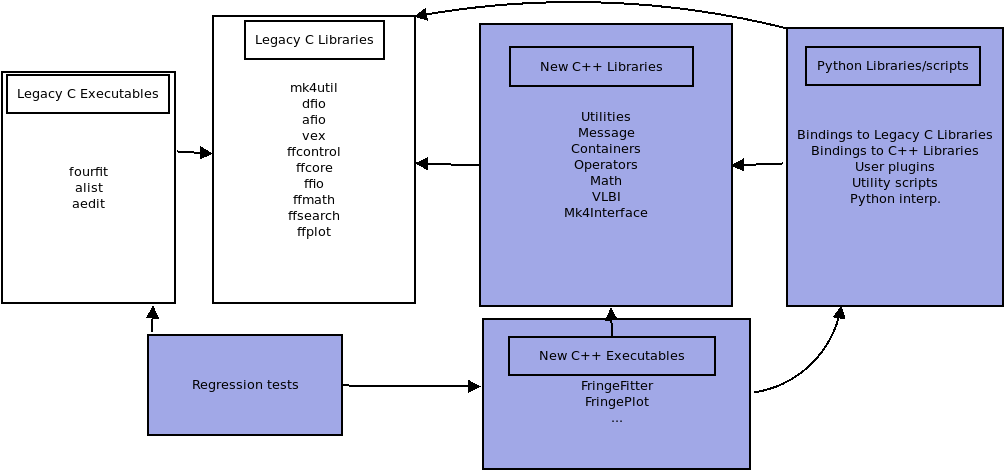
\includegraphics[width=0.95\textwidth]{fig/arch_overview.png}
    \caption{Basic overview of library and executable dependency architecture. Arrows indicate direction of dependency (from child to parent). Shaded boxes are new to-be-developed software.}
    \label{fig:lib-arch}
\end{center}
\end{figure}


\subsection{Executables}

The executables to be delivered will largely be composed through the re-use of the library code and at a minimum will consist of the following (though not necessarily
named as such):

\begin{enumerate}
 \item DiFX2Input  - difx2mark4 equivalent, converts correlator (difx) data into native input format.
 \item Station utilities  - converts station calibration data (e.g. ANTAB) files into native input format.
 \item FringeFitter - fourfit-replacement, accepts a user script (or old-style control file backwards compatibility) for configuration and direction and applies user specified procedures to the visibility data.
 \item FringePlot  - plotting tool, creates fringe-plots and all graphical data exploration.
 \item HDF5Export  - converts any native formats into an HDF5 format for access by external programs.
 \item DataInspect - data inspection tool, dumps data objects to a human readable format.
 \item alist - data inspection tool, dumps simple fringe summary data to a human readable format (as in HOPS3).
 \item aedit - data inspection/visualization tool (re-coded in python), reads alist files and provides simple plots of multiple scan data (as in HOPS3).
 \end{enumerate}
